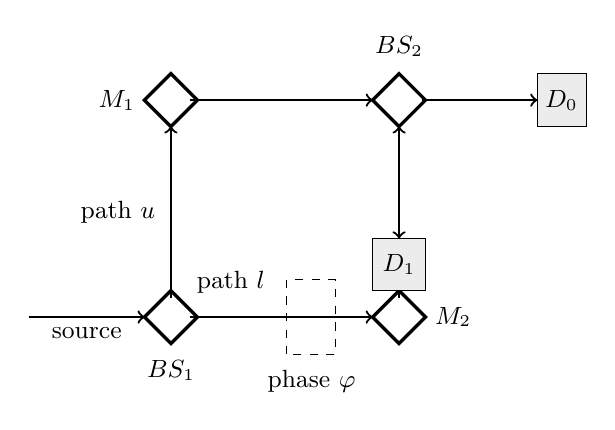
\begin{tikzpicture}[scale=0.95, every node/.style={font=\small}]
    \draw[->, thick] (-0.4,0) -- (1.15,0) node[midway, below] {source};
    \draw[very thick, rotate around={45:(1.5,0)}] (1.25,-0.25) rectangle (1.75,0.25);
    \node[below] at (1.5,-0.45) {$BS_1$};

    \draw[->, thick] (1.75,0) -- (4.2,0);
    \node[above] at (2.3,0.18) {path $\ket{l}$};
    \draw[->, thick] (1.5,0.25) -- (1.5,2.55) node[midway, left, xshift=-2pt] {path $\ket{u}$};

    \draw[very thick, rotate around={45:(1.5,2.9)}] (1.25,2.65) rectangle (1.75,3.15);
    \node[left] at (1.15,2.9) {$M_1$};
    \draw[->, thick] (1.75,2.9) -- (4.2,2.9);

    \draw[very thick, rotate around={45:(4.55,0)}] (4.3,-0.25) rectangle (4.8,0.25);
    \node[right] at (4.9,0) {$M_2$};
    \draw[->, thick] (4.55,0.25) -- (4.55,2.55);

    \draw[very thick, rotate around={45:(4.55,2.9)}] (4.3,2.65) rectangle (4.8,3.15);
    \node[above] at (4.55,3.35) {$BS_2$};

    \draw[->, thick] (4.85,2.9) -- (6.4,2.9);
    \draw[->, thick] (4.55,2.55) -- (4.55,1.05);
    \draw[fill=gray!15] (6.4,2.55) rectangle (7.05,3.25);
    \draw[fill=gray!15] (4.2,0.35) rectangle (4.9,1.05);
    \node at (6.72,2.9) {$D_0$};
    \node at (4.55,0.7) {$D_1$};

    \draw[dashed] (3.05,-0.5) rectangle (3.7,0.5);
    \node[below] at (3.38,-0.58) {phase $\varphi$};
\end{tikzpicture}
